
\section{Project Design}

I plan to used the data generated accordingly to the process described in Section \ref{Data}. I will also add new data sets, generated in the same manner to use as test/validation sets. The data needs to be explored and visualized to make sure all the chosen features can be used in the final analysis and if their behavior is performing as expected. Figure \ref{fig:mom} shows an example of data visualization, we can see the reconstructed muon momentum in the proton decay and the neutrino background samples. The blue curve contains all events in the sample, including events that do not have a prompt-gamma or events where the Kaon has a different decay mode\footnote{That is the reason for the $\approx 475 \textrm{ MeV}$ bump.}. The green curve is the signal sample, as expected we can see the peak of the distribution at $\approx 240 \textrm{ MeV}$ and the red curve shows the background distribution. Also as expected, the background sample shows a continuous spectrum of momentum with no peak present. This illustrates the type of exploration necessary to understand the data and optimize the selection analysis based on its behavior.

\begin{figure}[h]
  \centering
  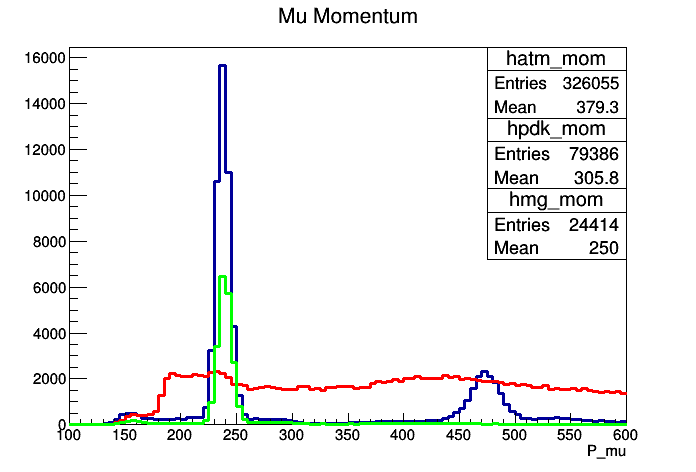
\includegraphics[width=0.6\linewidth]{figs/mom.png}
  \caption{Reconstructed muon momentum for all events in the proton decay sample (Blue), only the events that satisfy the signal requirement (Green) and the neutrino background sample (Red).}
  \label{fig:mom}
\end{figure}

After data exploration, I will pre-process the data to optimize the way classifiers work. For example, I can standardize all features so that all of them are dimensionless and have a similar magnitude. This way the classifier does not get tricked into thinking one variable is more important, for example the muon momentum, since it is a hundred times higher than the photon momentum.

Once data is ready to be fed to the algorithms, I will test the performance of different classifiers like BTDs and SVMs using the metrics discussed in Section \ref{Metric}. The basic pipeline will be choosing a cross-validation scheme like train-test split or stratified k-fold and perform a grid search on hyper parameters of the algorithms. Once some set of parameter is found, we can compare different algorithms and the benchmark model presented in Section \ref{Benchmark}. Due to the fact that these comparisons will possibly use different metrics, I might revisit the parameter set to compare only with the benchmark, in case the number of FP needs to be reduced.

